\documentclass[a4paper,12pt]{article}
\usepackage[utf8]{inputenc}
\usepackage[T2A]{fontenc}
\usepackage{amsmath}
\usepackage{hyperref}
\hypersetup{colorlinks=true}
\usepackage{colortbl}
\usepackage{graphicx}
\usepackage{float}
\usepackage{gensymb}
\pagecolor[rgb]{1,1,1}
%\pagecolor[rgb]{1,.98,.9}

\usepackage{titlesec}
\newcommand{\sectionbreak}{\clearpage}

\hypersetup{colorlinks=true, linkcolor=black}

\title{U{\degree}OS blockchain framework}
\author{}

\begin{document}

\clearpage\maketitle
\thispagestyle{empty}
%\maketitle


\clearpage\tableofcontents
\setcounter{page}{1}
%\thispagestyle{empty}


\clearpage
%\setcounter{page}{1}
\begin{abstract}

The concept of a cryptographically protected and distributed transaction ledger has demonstrated its efficiency in a series of projects. Decentralized frameworks based on blockchain technology allow communities to build transparent and reliable P2P systems that implement economic relationships between the users of the network. Over the recent years a series of consensus protocols were created and utilized in existing blockchain systems \textcolor{blue}{[citations]}. In this paper we introduce the U{\degree}OS blockchain framework and a novel DPoI (Delegated Proof of Importance) consensus algorithm that takes into consideration the value of the social and economic interactions between the members of the community and motivates users to actively contribute to the network growth. Notably, our DPoI metric can be modified to account for a variety of interactions, that arise in a particular network system. DPoI is a high-performance, resource efficient, network-growth inducing algorithm that rewards network participants for the economy enhancing operations in the system. Delegated Proof of Importance is an upgrade to the existing blockchain solutions, that integrates the concepts of the Delegated Proof of Stake (DPoS) and properties of networks. The system protocol is designed in accordance with business and end-user requirements such as privacy, transparency, and smooth volatility, which is achieved due to adaptive emissions proportionate to both network activity growth and the volume of the network itself, according to Metcalfe's law \cite{Metcalfe}. Our U{\degree}OS blockchain framework with the DPoI consensus metric represents a flexible architecture that can be deployed to set up a number of decentralized blockchain-based applications from social networks to service platforms with the direct growing economic value for all users. In this sense, U{\degree}OS is a unique framework that unlike any centralized system can be employed to create highly transparent community-based economies.



\end{abstract}

\section{Introduction}

An unprecedented growth of interest in blockchain technologies has been observed in the recent years \textcolor{blue}{[citations]}. At this time these technologies were primarily implemented in the form of distributed payment networks \textcolor{blue}{[citations]}. These networks are decentralized and enable fast low-cost P2P financial transactions between the users of the system. The basis of any blockchain that determines its technical characteristics is the network consensus algorithm. Namely, the consensus algorithm is the mechanism that allows the network nodes to reach consensus about the contents of a distributed ledger. In this paper we would like to review existing consensus protocol solutions and introduce a novel U{\degree}OS blockchain framework with a corresponding DPoI consensus metric. DPoI metric stimulates user involvement in the network growth via social and economic interactions, while allowing for an adjustable method of quantification of the user’s contribution to the community.


\subsection{Previous work}

The problem of distributed consensus for networks with potentially fraudulent participants known as the Byzantine Generals' Problem was stated in 1982, long before the creation of blockchain. \cite{Lamport} Since then an array of different solutions has been developed \cite{Castro}. However, the first solution that did not rely on a trusted third party, was the Proof-of-Work (PoW) algorithm \cite{satoshi}. Despite its advantages, PoW inherently has a number of shortcomings, namely, security \cite{Eyal}, scalability, performance\cite{Croman}, the problem of progressive centralization of the networks around the largest mining pools \cite{Buterin} and, most importantly, the need to use vast volumes of physical resources, such as electricity and computing power to generate blocks. \cite{Bentov}. 

Computing resources needed for hashing blocks in current blockchain frameworks, that implement PoW, are tremendous and far exceed the computing power of the world’s greatest supercomputers. Energy use for the block mining is comparable to the power consumption of some countries and it continues to grow \cite{energy}. In 2012, in order to mitigate these shortcomings, the PPCoin, currently  known as PeerCoin, cryptocurrency became the first to utilize an alternative consensus algorithm, Proof-of-Stake (PoS) \cite{Ppcoin}. In PoS consensus networks, the probability of creating a new block depends on the volume of tokens in a participant’s account. Despite significant reduction in resource utilization, PoS turns out to have several drawbacks and in its current state, according to a number of experts, cannot serve as an adequate replacement to PoW \cite{Demeester}, \cite{Poelstra}. One of the major weaknesses of PoS is that it additionally motivates users to concentrate all funds in one place or with one user, which leads to centralization of the network. The next iteration of PoS was introduced as the Delegated Proof-of-Stake (DPoS) \cite{dantheman}. Here network members are divided into two groups: members, who delegate the authority to create blocks and validate transactions, and validators (block producers). This partition provides better scalability and efficiency. Nevertheless, DPoS still has the problem of motivation for a participant to use their assets actively instead of accumulating them, which has a negative impact on the growth and governability of the network. Yet another consensus metric, the Proof-of-Importance consensus algorithm (PoI), was first introduced in the NEM cryptocurrency \cite{nem}. PoI incentivizes network participants' activity. The major departure from PoS is that block generation probability and reward distribution depends not only on the volume of a user's deposits, but also on the participant's activity rate and reputation. Thus, the algorithm motivates users to be more active by participating in more transactions and contributing to the network growth. Despite all its merits, PoI has some shortcomings in efficiency.\textcolor{red}{Comment: details about the shortcomings - Lesha didn't write this sentence, I think it needs a little more explanation.}


\subsection{Motivation}
As a matter of fact, social and economic interactions are integral components of any network system. Therefore, facilitation of social and economic activities contributes to the network development. We propose here a novel DPoI consensus algorithm that takes into account users' social and financial transactions in order to encourage participation in the network growth and prevent centralization. U{\degree}OS framework with DPoI consensus algorithm allows users to build virtually any network economy system on top of the U{\degree}OS blockchain and assign flexible financial and social activity scores, that reflect the nature of the socio-economic relationships in that particular system. 


\section{U{\degree}OS consensus algorithm}

The major goal of U{\degree}OS project is to design a consensus algorithm with an individual influence score metric, that facilitates efficient score redistribution, motivates users to participate actively in the network development and prevents centralization. Modern blockchain solutions have problems with scalability, security and efficiency, and to solve those problems, U{\degree}OS protocol introduces the DPoI (Delegated Proof of Importance) Consensus Algorithm. This consensus algorithm combines the advantages of DPoS and PoI and implements a new feature of delegating validation rights to a limited number of accounts in order to achieve high levels of efficiency and scalability within the network, accounting for transactional activity of the protocol members, and leading to its further development. 


The U{\degree}OS consensus algorithm (Delegated Proof-of-Importance, DPoI) is based on the DPoS consensus algorithm, implemented in the EOS blockchain \textcolor{blue}{[citation]}. In addition to the client's stake amount, our algorithm also considers the client's financial and social transactional activities. In the U{\degree}OS Protocol participants have the option of delegating the right to validate blocks to a limited number of accounts through voting, using their personal importance scores, analogous to EOS system. Unlike DPoS score, however, DPoI importance score formula is calculated from three components, namely, the stake amount, financial transfer activity and social activity. This framework is highly flexible since the network can control not only the weight of contribution of each term in the final importance score, but also choose how to calculate the transfer and social activity scores, given the structure of economic and social interactions in the system. To prevent activity imitation or fraud between several affiliated accounts, the transactional graph is partitioned into clusters using the SCAN algorithm \cite{SCAN}. In general, the working principle of the U{\degree}OS Protocol Consensus Algorithm can be explained as follows. 


\subsection{Importance score calculation}

DPoI importance score can be interpreted as an importance rating of an account \textit{i} in the network. It is calculated as follows: 

\begin{equation}
    \label{importance_rating}
    r_i = (1 - \omega_a - \omega_s) v_i + \omega_a \pi_i + \omega_s \sigma_i
\end{equation}
where $v_i$ is the stake volume index, $\pi_i$ is the financial activity index, $\sigma_i$ is the social network activity index, and $\omega_a$ and $\omega_s$ are the weight coefficients, that determine the relative significance of each component of the user activity. 

Stake volume index is based on the amount of tokens owned by the account, and represents balance proportion of the total amount of tokens in the system. Thus, an account with non-zero balance has non-zero importance index. Social and financial activity indices depend on the transactional history of the account. These indices are calculated using NCDAwareRank algorithm, described in the details in the sections below. Noticeably, each network application based on U{\degree}OS framework can define their unique set of financial and social transactions that are included in the calculation of the corresponding financial and social index scores. These programs can be integrated with the U{\degree}OS blockchain as DApps (distributed applications) and implement a wide range of economic and/or social systems, such as service platforms, knowledge networks, digital content copyright systems, libraries, public records, online markets etc. Unlike centralized versions of such services, U{\degree}OS DApps would preserve the important properties of blockchain decentralized systems, particularly, \textcolor{red}{Comment: what are the most important properties of blockchain apart from transparency and immutability? and also stress economic incentrive for all users of the network here again}

Financial and social activity indices, $\pi_i$ and $\sigma_i$ are calculated according to the NCDAwareRank algorithm. We will describe the main principles of the algorithm, based on the calculation of the financial index $\pi_i$. Later in the separate section we will explain how the algorithm is used to calculate the social activity component $\sigma_i$.  NCDAwareRank gives more preference to the accounts that are tightly integrated in the general network, which helps to make the network resistant to splitting account attacks. Another important feature of the algorithm is the utilization of incoming activity only. This is a PageRank-based paradigm, namely, a user cannot obtain the score from the existing account. Such a score is a direct representation of the user's utility for the entire network.

%Activity index is calculated only for accounts with the balance exceeding the $A_0$ threshold. This value is not fixed and is determined by committee members. When calculating the account activity index only transactions with the amount of tokens higher than $T_0$ are taken into account. That value is also determined by the committee. Hidden transactions are not included. Activity index depends on transactions, creation time of which lays in some time interval. The duration of this interval is $W$ blocks. Contribution of every transaction decreases exponentially.


\subsubsection{Financial activity score calculation}
The vector of financial indices $\boldsymbol{\pi^{(j)}}$, where $j$ is the indicator of the iteration in the algorithm, is calculated following the recurrent relation: 

\begin{equation}
    \label{recurrent_formula_for_ncdawarerank}
    \boldsymbol{\pi}^{(j+1)} = ( \eta \boldsymbol{O} + \mu \boldsymbol{M} + ( 1 - \eta - \mu ) \boldsymbol{E} ) \boldsymbol{\pi}^{(j)}
\end{equation}

Here $\boldsymbol{\pi^{(j)}}$ is a vector of account importance indexes values. The vector is normalized, i.e. the sum of its elements is 1. $\boldsymbol{O}$ is the outlink matrix, $\boldsymbol{M}$ is the interlevel proximity matrix. See the definitions of the matrices below. $\eta$ and $\mu$ are weight coefficients that determine contributions of the $\boldsymbol{O}$ and $\boldsymbol{M}$ matrices. Their sum must be less than 1. $\boldsymbol{E}$ is the teleportation matrix added to ensure the series is convergent. This is defined as follows:
$$
\boldsymbol{E}=\frac{1}{N}\boldsymbol{e}
$$
where \textit{N} is the number of the accounts and $\boldsymbol{e}$ is the matrix in which all the elements are equal to 1, the calculation continues until for some i the following condition is fulfilled: 



$$
\lVert \boldsymbol{\pi}^{(j+1)}-\boldsymbol{\pi}^{(j)} \rVert <\varepsilon
$$

Here $\lVert \cdot \rVert$ is the vector norm defined as the sum of its elements, $\varepsilon$ is the predetermined calculation accuracy. As an initial approximation, a vector $\boldsymbol{\pi^{(0)}}$ with all the elements equal to $\frac{1}{N}$ can be used.



\paragraph{Outlink matrix calculation}

The outlink matrix $O$ is calculated as follows: First the weight matrix is calculated:



$$
w_{ij}=\sum_{k|i \to j, {h_k \ge H_0} \land {h_k \le H_0+W}} \theta ( a_k - T_0 ) \theta ( s_i - A_0 ) \theta ( s_j - A_0 ) a_k \exp{(lnK [\frac{h_k}{D}])}
$$

where $a_k$ is the sum of transaction \textit{k}, $h_k$ is the transaction depth (the block order number from the current point, also known as a block height),  $K$ and $D$ are transaction contribution decrease parameters, that define how much the contribution of each transaction decreases over time. The purpose of these parameters is that over every $D$ number of blocks, created after the given transaction, the transaction contribution decreases by $w'=Kw$. The sum is taken over all the transactions of a deposit from account \textit{i} to account \textit{j}, depth of which lays between $H_0$ and $H_0+W$. $H_0$ and $W$ are parameters, its values are equal $H_0=2419200$ and $W=1000$ currently in the testnet. So, only transactions from time gap, duration of which is $W$ blocks, contribute to activity index.







$$
\hat{o}_{ij} = \begin{cases}
 w_{ji}-w_{ij}
 & \text{if $w_{ji}-w_{ij} > 0$,}\\
 0 & \text{otherwise.}
\end{cases}
$$

Then the matrix that was obtained  is normalized so that the sum of elements in every column is equal to 1.


$$
o_{ij} = \begin{cases}
 \frac{\hat{o}_{ij}} {\sum\limits_{k} \hat{o}_{kj}}
 & \text{if $\sum\limits_{k} \hat{o}_{kj}> 0$,}\\
 0 & \text{otherwise}
\end{cases} 
$$

\paragraph{Interlevel proximity matrix calculation}

Let W is a set of all the accounts taken into the Importance Index calculation; W is a set divided into disjoint subsets $A_i$ called NCD-blocks (Nearly Completely Departed). See the SCAN algorithm description for details. For the given “account u”, “$G_u$” is the set of all the accounts, for which the according member of outlink matrix is greater than zero: $o_{uv} > 0$. Then the set of proximal “accounts u” is defined as follows: 



$$
\chi_u = \bigcup_{v \in \{u\} \cup G_u} A_{(v)}
$$

The interlevel proximity matrix is defined as follows:



$$
M_{vu}=\begin{cases}
 \frac{1}{N_u |A_{(v)}|}
 & \text{if $v \in \chi_u$ ,}\\
 0 & \text{otherwise.}
\end{cases}
$$

Where $N_u$ is the number of NCD-blocks in $\chi_u$.



\paragraph{SCAN algorithm based graph partitioning into clusters}

An indirected graph $W = \{V, E\}$ has every vertex representing a client, and every edge representing a non-zero element of the outlink matrix. The structure of the vertex $v$ is the set of all the adjacent vertices:


$$
\Gamma(v)=\{w \in V|(v,w) \in E\} \cup \{v\}
$$

The structural similarity of two vertices can be defined as follows:



$$
\sigma(v,w)=\frac{ |\Gamma(v) \cap \Gamma(w)|}{\sqrt{|\Gamma(v)||\Gamma(w)|}}
$$

The vertex $\varepsilon$-neighborhood is a set of vertices for which


$$
N_{\varepsilon}(v) = \{ w \in \Gamma(v) | \sigma(v,w) \ge \varepsilon \}
$$

The \textit{CORE} is a vertex for which the number of elements in the $\varepsilon$-neighborhood is more than $\mu$.

$$
CORE_{\varepsilon,\mu}(v) \Leftrightarrow |N_{\varepsilon} (v)| \ge \mu
$$

Vertex $w$ is directly structurally reachable from vertex $v$ if



$$
DirREACH(v,w) \Leftrightarrow CORE_{\varepsilon,\mu}(v) \vee w \in N_{\varepsilon}(v)
$$

Vertex $w$ is structurally reachable from vertex $v$ if


$$
REACH(v,w) \Leftrightarrow \exists v_1,...v_n \in V \forall i \in \{1,...n-1\}DirREACH(v_i,v_{i+1})
$$

Vertex $v$ is structurally connected with vertex $w$ if



$$
CONNECT(v,w) \Leftrightarrow \exists u \in V REACH(u,v) \vee REACH(u,w)
$$

A cluster is a subset of vertices structurally connected to each other. It is possible to show that every vertex can only belong to one cluster. A vertex can also belong to no cluster; in this case it can either be a hub if there are vertices belonging to two different clusters in its environment, otherwise it is an independent vertex.


%\begin{figure}[h]
 %     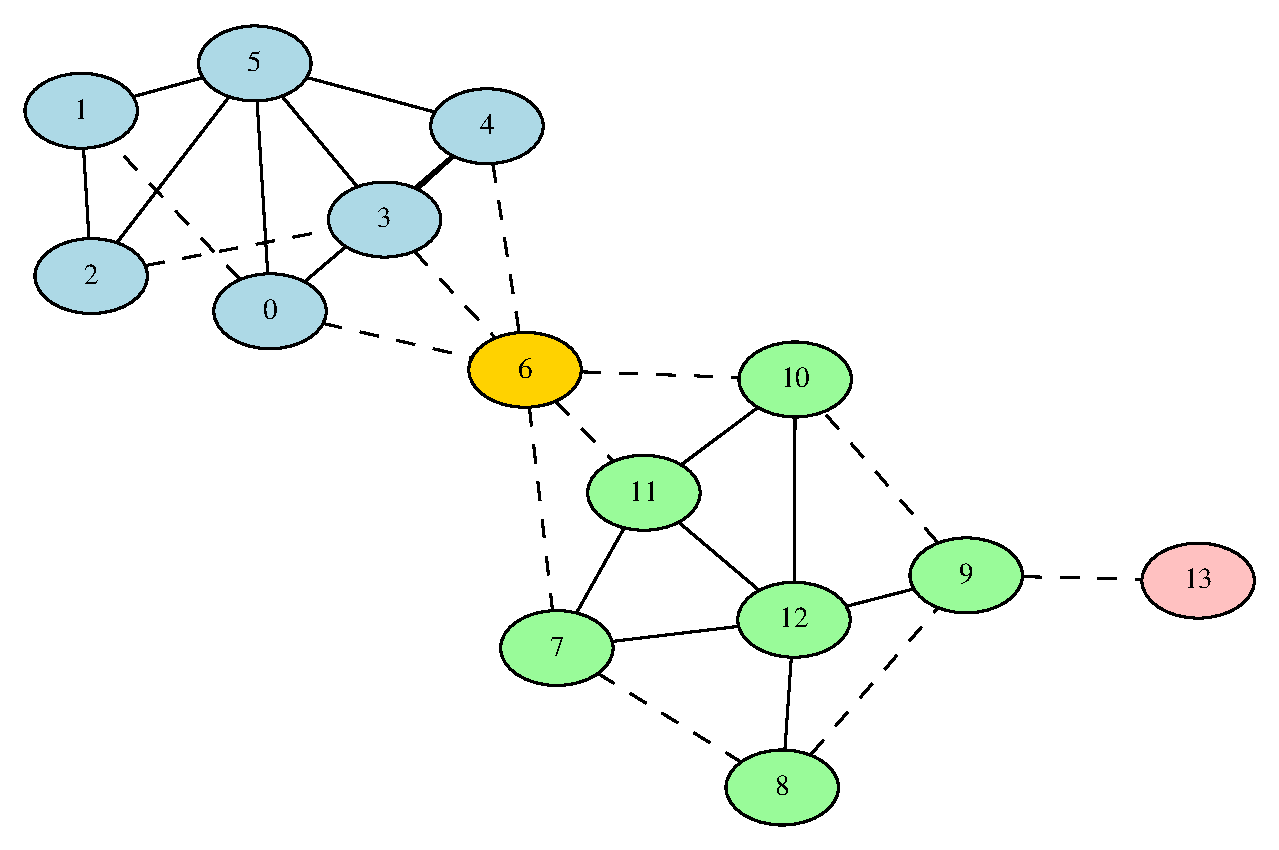
\includegraphics[width=1\linewidth]{pictures/clustering_example.eps}
   %   \caption{SCAN algorythm applying example. Parameters $\varepsilon=0.7$ and $\mu=4$ were used.}
     % \label{fig:sigmoida}
%\end{figure}


\subsubsection{Social activity score calculation}
\textcolor{red}{Comment: Lesha will be commiting a new version of the library that calculates the score, and update for this section this week, I think, so I can build this section upon the changes that he made}


\subsection{Importance score usage}

Importance index $r_i$ in the framework is used for two major purposes:
\begin{itemize}
\item emission calculation for each user \textit{i}
\item  network governance through voting for validators (block producers) and committee members
\end{itemize}

 %user rankings is not a part of the algorithm

First, it defines the amount of new tokens which every account receives in case the emission is positive.  

Second, importance index defines the account’s weight during the voting. The voting allows the delegation of certain powers within the system to a limited number of the validation accounts. Producers who own nodes that produce and verify blocks are selected by voting.

Members of the committee are also selected by voting. The committee can vote on blockchain settings, such as the fee amount for a transaction, producer node reward and so on. 


\subsection{Key features of the algorithm}
\textcolor{red}{Comment: here we describe key advantages of the system and the algorithm, in particular, the features that make the algorithm more resistant to attacks, are there any other notable technical fetures that we want to highlight?}

Following mitigations are used in the project, in order to reduce the risk of attacks.

\begin{itemize}
  \item Only incoming transfers contribute to importance index, it makes obtaining score from existing accounts more difficult.
  \item There are stake threshold for accounts, participating in importance index calculation, and amount threshold fot transfers. It makes attacks more expensive for attackers.
  \item Using NCDAwareRank instead of PageRank makes the system more resistant to splitting account attacks. This algorythm gives preference to accounts, tightly integrated to common network.
  \item Coefficients $\omega_a$ and $\omega_s$ have relatively small values, it makes contribution of activity index and social index to total importance index significantly less than stake contribution.
  \item Using decaying weights makes effect of any fraud activity temporary. Stopping fraud activity causes quick decreasing obtained score.
\end{itemize}


\section{Emission}

\subsection{U{\degree}OS token utilization}

\textcolor{red}{Comment: talk to Sasha Spirin and others -- it is not yet clear if this section belongs to the paper.}
%The amount of transactions processed directly depends on the available computing power provided by network members. To allocate the resources efficiently and to avoid spam attacks, a fee in the protocol core cryptographic token is levied on the operations within the U{\degree}OS network. The protocol allows a user to make token transfer transactions between the network members and launch system smart contracts, e.g. multi-signature, account registration, user tokens creation and so on.

Emission amount at launch is 1,000,000,000 protocol tokens, distributed to the original network accounts to start the protocol. The U{\degree}OS project implements adaptive emission. The emission volume is calculated regularly once, in a certain time interval, $t_0, t_1, ... t_i$, where $t_{i+1} = t_i + T$. The volume of emission depends on the network activity growth in the preceding time period $T$.


\subsection{Calculating network activity for a period of time}

To begin, we calculate the matrix of weights according to the formula:



$$
w_{ij}(t_n)=\sum_{k|i \to j, t_k \in [t_{n-1}, t_n]}a_k
$$

Here $a_k$  is the amount in k-th transaction, $t_k$  the time at which k-th transaction was created. Summation is performed for all the transactions transferring any amount from account $i$ to account $j$ and created at the time frame from $t_{n-1}$ to $t_n$. 

In fact, each matrix element $w_{ij}$ represents a weight of connection between account $i$ and account $j$ in a given time frame. Next we need to calculate the matrix of connections $l$: 



$$
l_{ij}(t_n) = \begin{cases}
 1
 & \text{if $w_{ji}(t_n)-w_{ij}(t_n) > 0$,}\\
 0 & \text{otherwise.}
\end{cases}
$$

We calculate the activity in a given time frame as:



$$
A(t_n) = \sum_{i,j} l_{ij}(t_n)
$$

In this way, activity is calculated as a number of connections between active accounts in a set timeframe. 



\subsection{Emission value calculation}

Emission value depends on network activity growth.

$E_T$ value is defined as follows, and it is the target value of emission. It defines the upper bound of the aggregate amount of the emission, that is achievable with the following activity value $A$:



$$
\Delta A(t_n) = A(t_n) - A_{max}(t_{n-1})
$$

$$
E_T(t_n) = \begin{cases}
 E_T(t_{n-1}) + K_E \Delta A(t_n),
 & \text{when $\Delta A(t_n) > 0$,}\\
 E_T(t_{n-1}) & \text{otherwise}
\end{cases}
$$

Here $K_E$ is a coefficient which defines the maximum value of the emission with activity increased by 1. $A_{max}(t_{n-1})$ is the previous maximum value since the system launch:



$$
    A_{max}(t_{n-1}) = max \Big ( A(t_i), t_i \in [t_0, t_{n-1}] \Big )
$$

Emission value, which is issued at a certain time $t_n$, is defined by formula:



$$
    E(t_n) = \lambda S(t_{n-1}) f \Big( \kappa \frac {E_T(t_n) - E_S(t_{n-1})}{\lambda S(t_{n-1})} \Big)
$$

Here $\lambda$ is the marginal growth of the token amount in the system S per one emission. It is defined through $L$, which specifies the marginal growth $S$ in a year, expressed as a percentage:



$$
    \lambda = (1 + \frac{L}{100})^{1/N}-1
$$

Here $N$ is the number of emission issues per year.



$f(x)$ - sigmoidal function (Fig \ref{fig:sigmoida}). In the present implementation of the algorithm a hyperbolic tangent is used as this function. 


$\kappa$ is a coefficient between 0 to 1 and it defines the speed at which a full emission approaches the target emission $E_T$ if the activity level remains the same over the long term.



Initial values of both $E_T$ and $E_S$ are zero:



$$
E_T(t_0)=0, E_S(t_0)=0
$$


%\begin{figure}[h]
 %     \includegraphics[width=1\linewidth]{pictures/sigmoida.eps}
  %    \caption{Sigmoidal function}
   %   \label{fig:sigmoida}
%\end{figure}


\section{U{\degree}OS framework architecture}
\textcolor{red}{Here we describe the systems architecture and maybe we should include the details of licensing and deployment.}


\addcontentsline{toc}{section}{Appendix 1 Glossary of terms}

\section*{Appendix 1 Glossary of terms}
\textbf{U{\degree}OS consensus algorithm (Delegated Proof-of-Importance, DPoI)}

The consensus algorithm, which is based on a calculation of the importance index of an account, which in turn depends on Stake Volume Index and Activity index

\textbf{Importance index}

The importance index of an account is calculated as a function of Stake Volume Index and Activity index

\textbf{Account}

An entity represented by a tuple of pairs of keys (public + private), which is registered in a blockchain by an individual.

\textbf{Producer}

Accounts with the right to verify blocks. They must have a node.

\textbf{Node}

A P2P network node, which performs all the calculations in blockchain. A node belonging to a producer account (producer node), produces blocks.


\addcontentsline{toc}{section}{References}
\begin{thebibliography}{99}
 \bibitem{Metcalfe} Metcalfe, B. (2013). Metcalfe's law after 40 years of ethernet. Computer, 46(12), 26-31. URL: http://ieeexplore.ieee.org/abstract/document/6636305/
 \bibitem{Lamport} Lamport, L., Shostak, R., Pease, M. (1982). The Byzantine generals problem. ACM Transactions on Programming Languages and Systems (TOPLAS), 4(3), 382-401. URL: https://www.microsoft.com/en-us/research/uploads/prod/2016/12/The-Byzantine-Generals-Problem.pdf
 \bibitem{Castro} Castro, M., Liskov, B. (2002). Practical Byzantine fault tolerance and proactive recovery. ACM Transactions on Computer Systems (TOCS), 20(4), 398-461. URL: https://dl.acm.org/citation.cfm?doid=571637.571640
 \bibitem{satoshi} Nakamoto, S. (2008). Bitcoin: A peer-to-peer electronic cash system. URL: https://bitcoin.org/bitcoin.pdf
 \bibitem{Croman} Croman, K. et al. (2016). On scaling decentralized blockchains. In International Conference on Financial Cryptography and Data Security (pp. 106-125). Springer, Berlin, Heidelberg. URL: http://www.comp.nus.edu.sg/~prateeks/papers/Bitcoin-scaling.pdf
 \bibitem{Eyal} Eyal, I., Sirer, E. G. (2014). Majority is not enough: Bitcoin mining is vulnerable. In International conference on financial cryptography and data security (pp. 436-454). Springer, Berlin, Heidelberg. URL: https://arxiv.org/pdf/1311.0243.pdf
 \bibitem{energy} Bitcoin Energy Consumption Index. digiconomist.net. URL: https://digiconomist.net/bitcoin-energy-consumption
 \bibitem{Buterin} Buterin, V. (2014). Mining Pool Centralization at Crisis Levels. URL: https://bitcoinmagazine.com/articles/mining-pool-centralization-crisis-levels-1389302892/
 \bibitem{Bentov} Bentov, I., Gabizon, A., Mizrahi, A. (2016). Cryptocurrencies without proof of work. In International Conference on Financial Cryptography and Data Security (pp. 142-157). Springer, Berlin, Heidelberg. URL: https://link.springer.com/chapter/10.1007/978-3-662-53357-4\_10/
 \bibitem{Ppcoin} King, S., Nadal, S. (2012). Ppcoin: Peer-to-peer crypto-currency with proof-of-stake. URL: https://peercoin.net/assets/paper/peercoin-paper.pdf
 \bibitem{Demeester} Demeester, T. (2017). Critique of Buterin’s A Proof of Stake Design Philosophy. URL: https://medium.com/@tuurdemeester/critique-of-buterins-a-proof-of-stake-design-philosophy-49fc9ebb36c6
 \bibitem{Poelstra} Poelstra, A. (2014). Distributed consensus from proof of stake is impossible. URL: https://download.wpsoftware.net/bitcoin/old-pos.pdf
 \bibitem{dantheman} Dantheman. (2017). DPOS Consensus Algorithm - The Missing White Paper. URL: https://steemit.com/dpos/@dantheman/dpos-consensus-algorithm-this-missing-white-paper
 \bibitem{nem} NEM Technical Reference. Version 1.2.1. February 23, 2018 URL: https://nem.io/wp-content/themes/nem/files/NEM\_techRef.pdf
\bibitem{SCAN} Xiaowei Xu et al. (2007). SCAN: A Structural Clustering Algorithm for Networks. URL: http://www1.se.cuhk.edu.hk/~hcheng/seg5010/slides/p824-xu.pdf
\end{thebibliography}

\end{document}